\chapter{Experimentos}
En este capítulo se describen los experimentos....

\section{Materiales}
     \subsection{Dispositivo para adquirir datos}
     Durante la etapa de adquisición de datos para el algoritmo de entrenamiento, además de conocer la ubicación de la persona y la de la figura que observan en pantalla es necesario capturar una imagen del rostro de la persona y conocer (mediante un aparato de medición) la orientación de la cabeza, lo anterior es necesario para evaluar y compararar el sistema de estimación de pose. \\
     Como señalan en [Murphy-Chutorian, 2009] el método que se utilice para obtener las medidas de la orientación de la cabeza en el conjunto de entrenamiento debe ser preciso y entre los métodos más eficientes proponen los sistemas captura ópticos de movimiento y los sensores inerciales, sin embargo, los primeros son muy costosos, por lo que en el desarrollo del presente trabajo de tesis se optó por utilizar un sensor inercial, el cual consiste de acelerómetros y giroscopios a menudo acoplados con algún tipo de filtro para reducir ruido.
     
     En este apartado se describirá el proceso de diseño y fabricación del dispositivo que realiza la medición de la orientación.\\
     De modo que la tarjeta electrónica debe ir en la cabeza de las personas, durante el diseño se tomó mucho en cuenta el tamaño y el peso que tendría, ya que de ser muy grande y  pesado podría ser muy incomodo para las personas durante los experimentos. 
     
     \subsubsection{IMU}
     El imu seleccionado para este proyecto es el BNO055 de Bosch (figura 5.1). El sensor utiliza algoritmos que mezclan los datos del acelerómetro, magnetómetro y giroscopio en una salida estable de la orientación de los tres ejes, el sensor es capaz de arrojar los datos en cuaterniones, vectores y ángulos de Euler. El BNO055 se alimenta con voltaje de 3.3 a 5v, mide 2.67x2.032cm y para obtener los datos utiliza comunicación I2C.
     
     \begin{figure}[htbp]
     	\centering
     	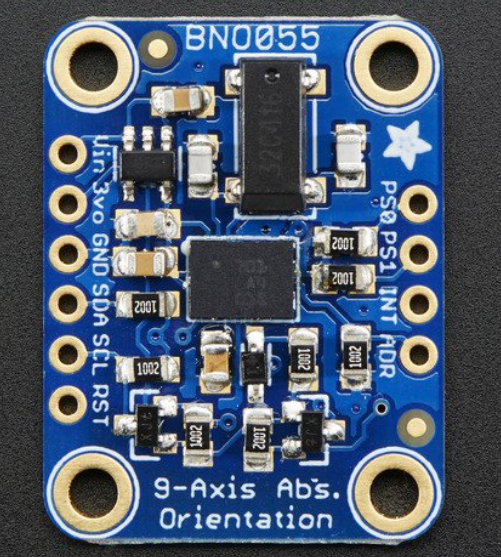
\includegraphics[width=0.25\textwidth]{./pictures/bno055}
     	\caption{}\label{fig: figura}
     \end{figure}
     
     \subsubsection{Microcontrolador}
     Debido a las restricciones de peso y tamaño se utilizó un arduino micro, el cual es la versión más pequeña del arduino con 4.8x1.8cm y esto se debe a que es una versión más limitada en cuanto a periféricos y módulos, sin embargo, es adecuada para el uso que se le da en el proyecto, únicamente se utilizará para obtener los datos del imu mediante comunicación I2C y enviarlos a la computadora por comunicación serial. El arduino se alimenta mínimo con 7v para que su regulador interno regule a 5v el microcontrolador que usa.
     \begin{figure}[htbp]
     	\centering
     	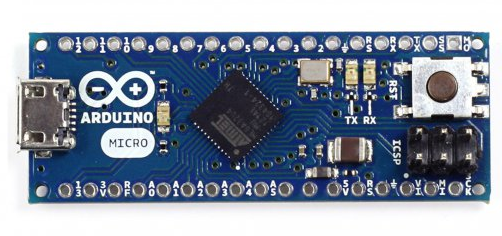
\includegraphics[width=0.4\textwidth]{./pictures/arduino}
     	\caption{}\label{fig: figura}
     \end{figure}
     
     \subsubsection{Xbee}
     Durante los experimentos las personas se estarán moviendo en diferentes posiciones de la escena y mirando diferentes lugares en la pantalla, como se había mencionado la tarjeta electronica se colocará en su cabeza, por lo que utilizar un cable (de comunicación serial) entre la computadora y la tarjeta para obtener los datos de la pose sería muy inadecuado ya que éste debe ser bastante largo, le pesaría a la tarjeta y afectaría su posición en la cabeza, y finalmente podría afectar la experiencia de la persona el tener un cable muy extenso cerca de ella. Tomando en cuenta las consideraciones anterior se decidión trabajar con módulos xbee.\\
     Los xbee son módulos inalámbricos creados para la comunicación inalámbrica entre ellos, su finalidad es la eliminación de cables en la comunicación serial. Para este proyecto se utilizaron los xbee s1 (figura 5.3) los cuales son los más  pequeños, de bajo consumo y simples de utilizar debido a que su configuración punto a punto es bastante sencilla y únicamente se requiere declarar un xbee como emisor y el otro como receptor. Los xbee s1 se alimentan con 3.3v.
     
     \begin{figure}[htbp]
     	\centering
     	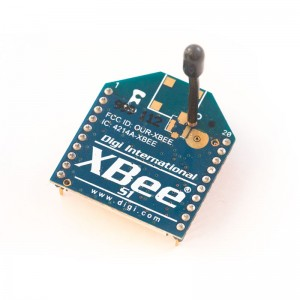
\includegraphics[width=0.3\textwidth]{./pictures/xbee}
     	\caption{}\label{fig: figura}
     \end{figure}
     
     \subsubsection{Diseño de la tarjeta}
     Para alimentar todo el circuito es necesario al menos 7v, ya que como se habíía mencionado eso necesita el Arduino micro y es el dispositivo que requiere mayor voltaje, el imu funciona con 5v por lo que se le puede conectar el pin de 5v que tiene el Arduino, sin embargo aún se tiene el inconveniente de que el xbee y su comunicación funcionan con 3.3v, y las baterías recargabales de iones de litio como la que se pretende utilizar por su reducido tamaño y peso, arrojan solo 3.7.v.\\
     Para solucionar el problema de los 7v se utilizó la bomba de carga TPS61093, figura 5.4, en una configuración para elevar el voltaje a 7v. La comunicación entre el arduino y el xbee (diferentes niveles de voltaje) se logró mediante el cambiador de nivel TXS0102, y finalmente para obtener 3.3v de la batería se utilizó el regulador TPS73633. Se pudo alimentar el xbee a través del pin de 3.3v del arduino, sin embargo, el xbee consume hasta 60mA lo cual es demasiado para el regulador de 3.3v del Arduino y podría afectar su funcionamiento.
     
     \begin{figure}[htbp]
     	\centering
     	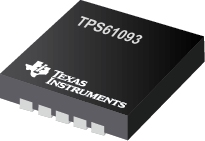
\includegraphics[width=0.15\textwidth]{./pictures/TPS61093}
     	\caption{}\label{fig: figura}
     \end{figure}
     En la imagen 5.5 se puede ver el esquemático de la tarjeta y en la 5.6 el pcb.
     \begin{figure}[htbp]
     	\centering
     	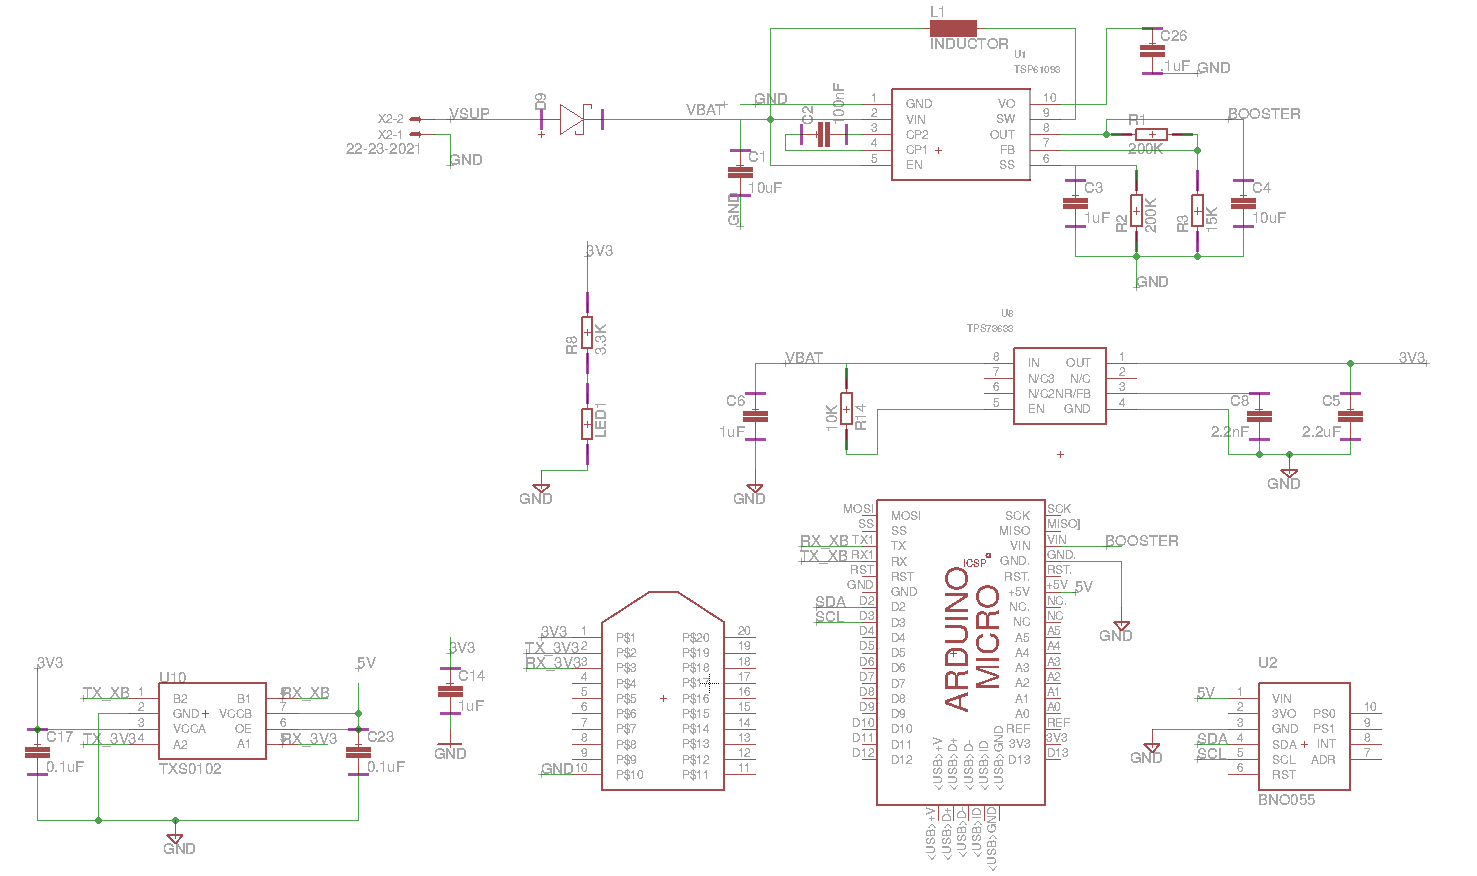
\includegraphics[width=1.\textwidth]{./pictures/schematic}
     	\caption{}\label{fig: figura}
     \end{figure}
     \begin{figure}[htbp]
     	\centering
     	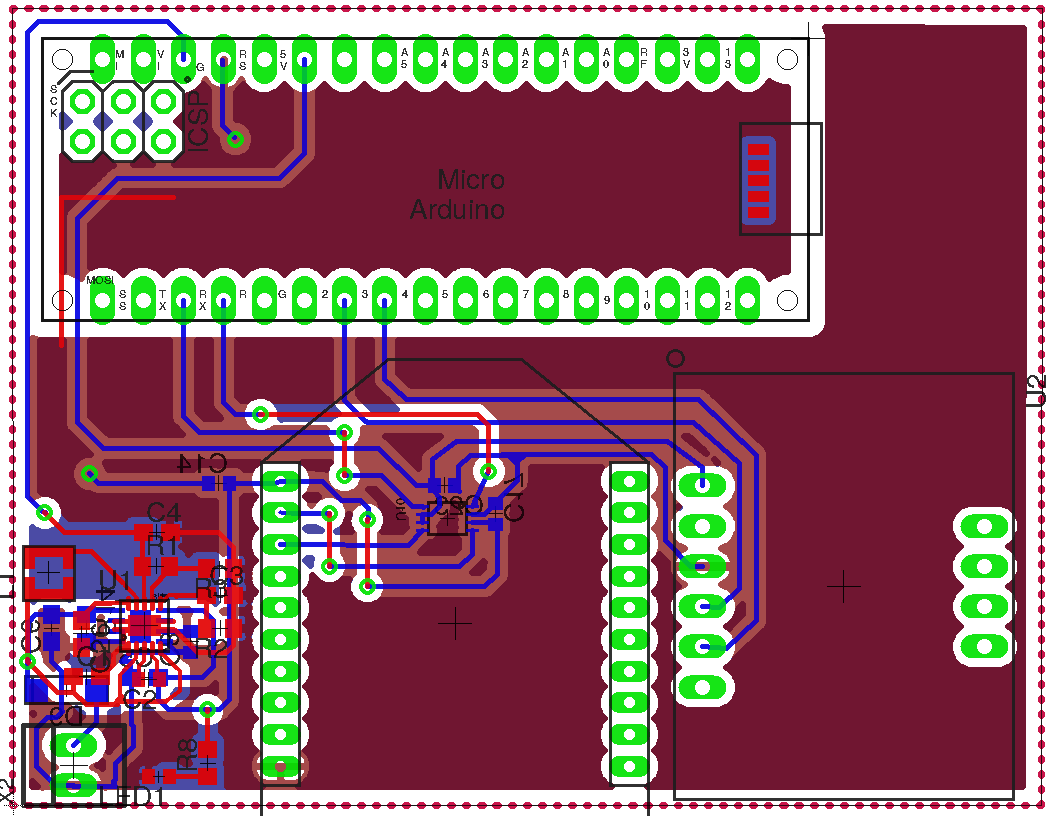
\includegraphics[width=1.\textwidth]{./pictures/board}
     	\caption{}\label{fig: figura}
     \end{figure}
     Adicionalmente se creo una pequeña tarjeta para la recepción de datos a través del otro xbee y envío a la computadora mediante un cable con convertidor de rs232 a usb. Más adelante se detallará el programa para la recepción de datos.
     
     \subsubsection{tarjeta electrónica}
     En las siguientes imágenes se presentan: la tarjeta electrónica con el imu, arduino y xbee ya fabricada; la batería recargable de 3.7v y la tarjeta que conecta el xbee receptor de datos con la computadora para poder enviar los datos del imu hacia la computadora.
     \begin{figure}[htbp]
     	\centering
     	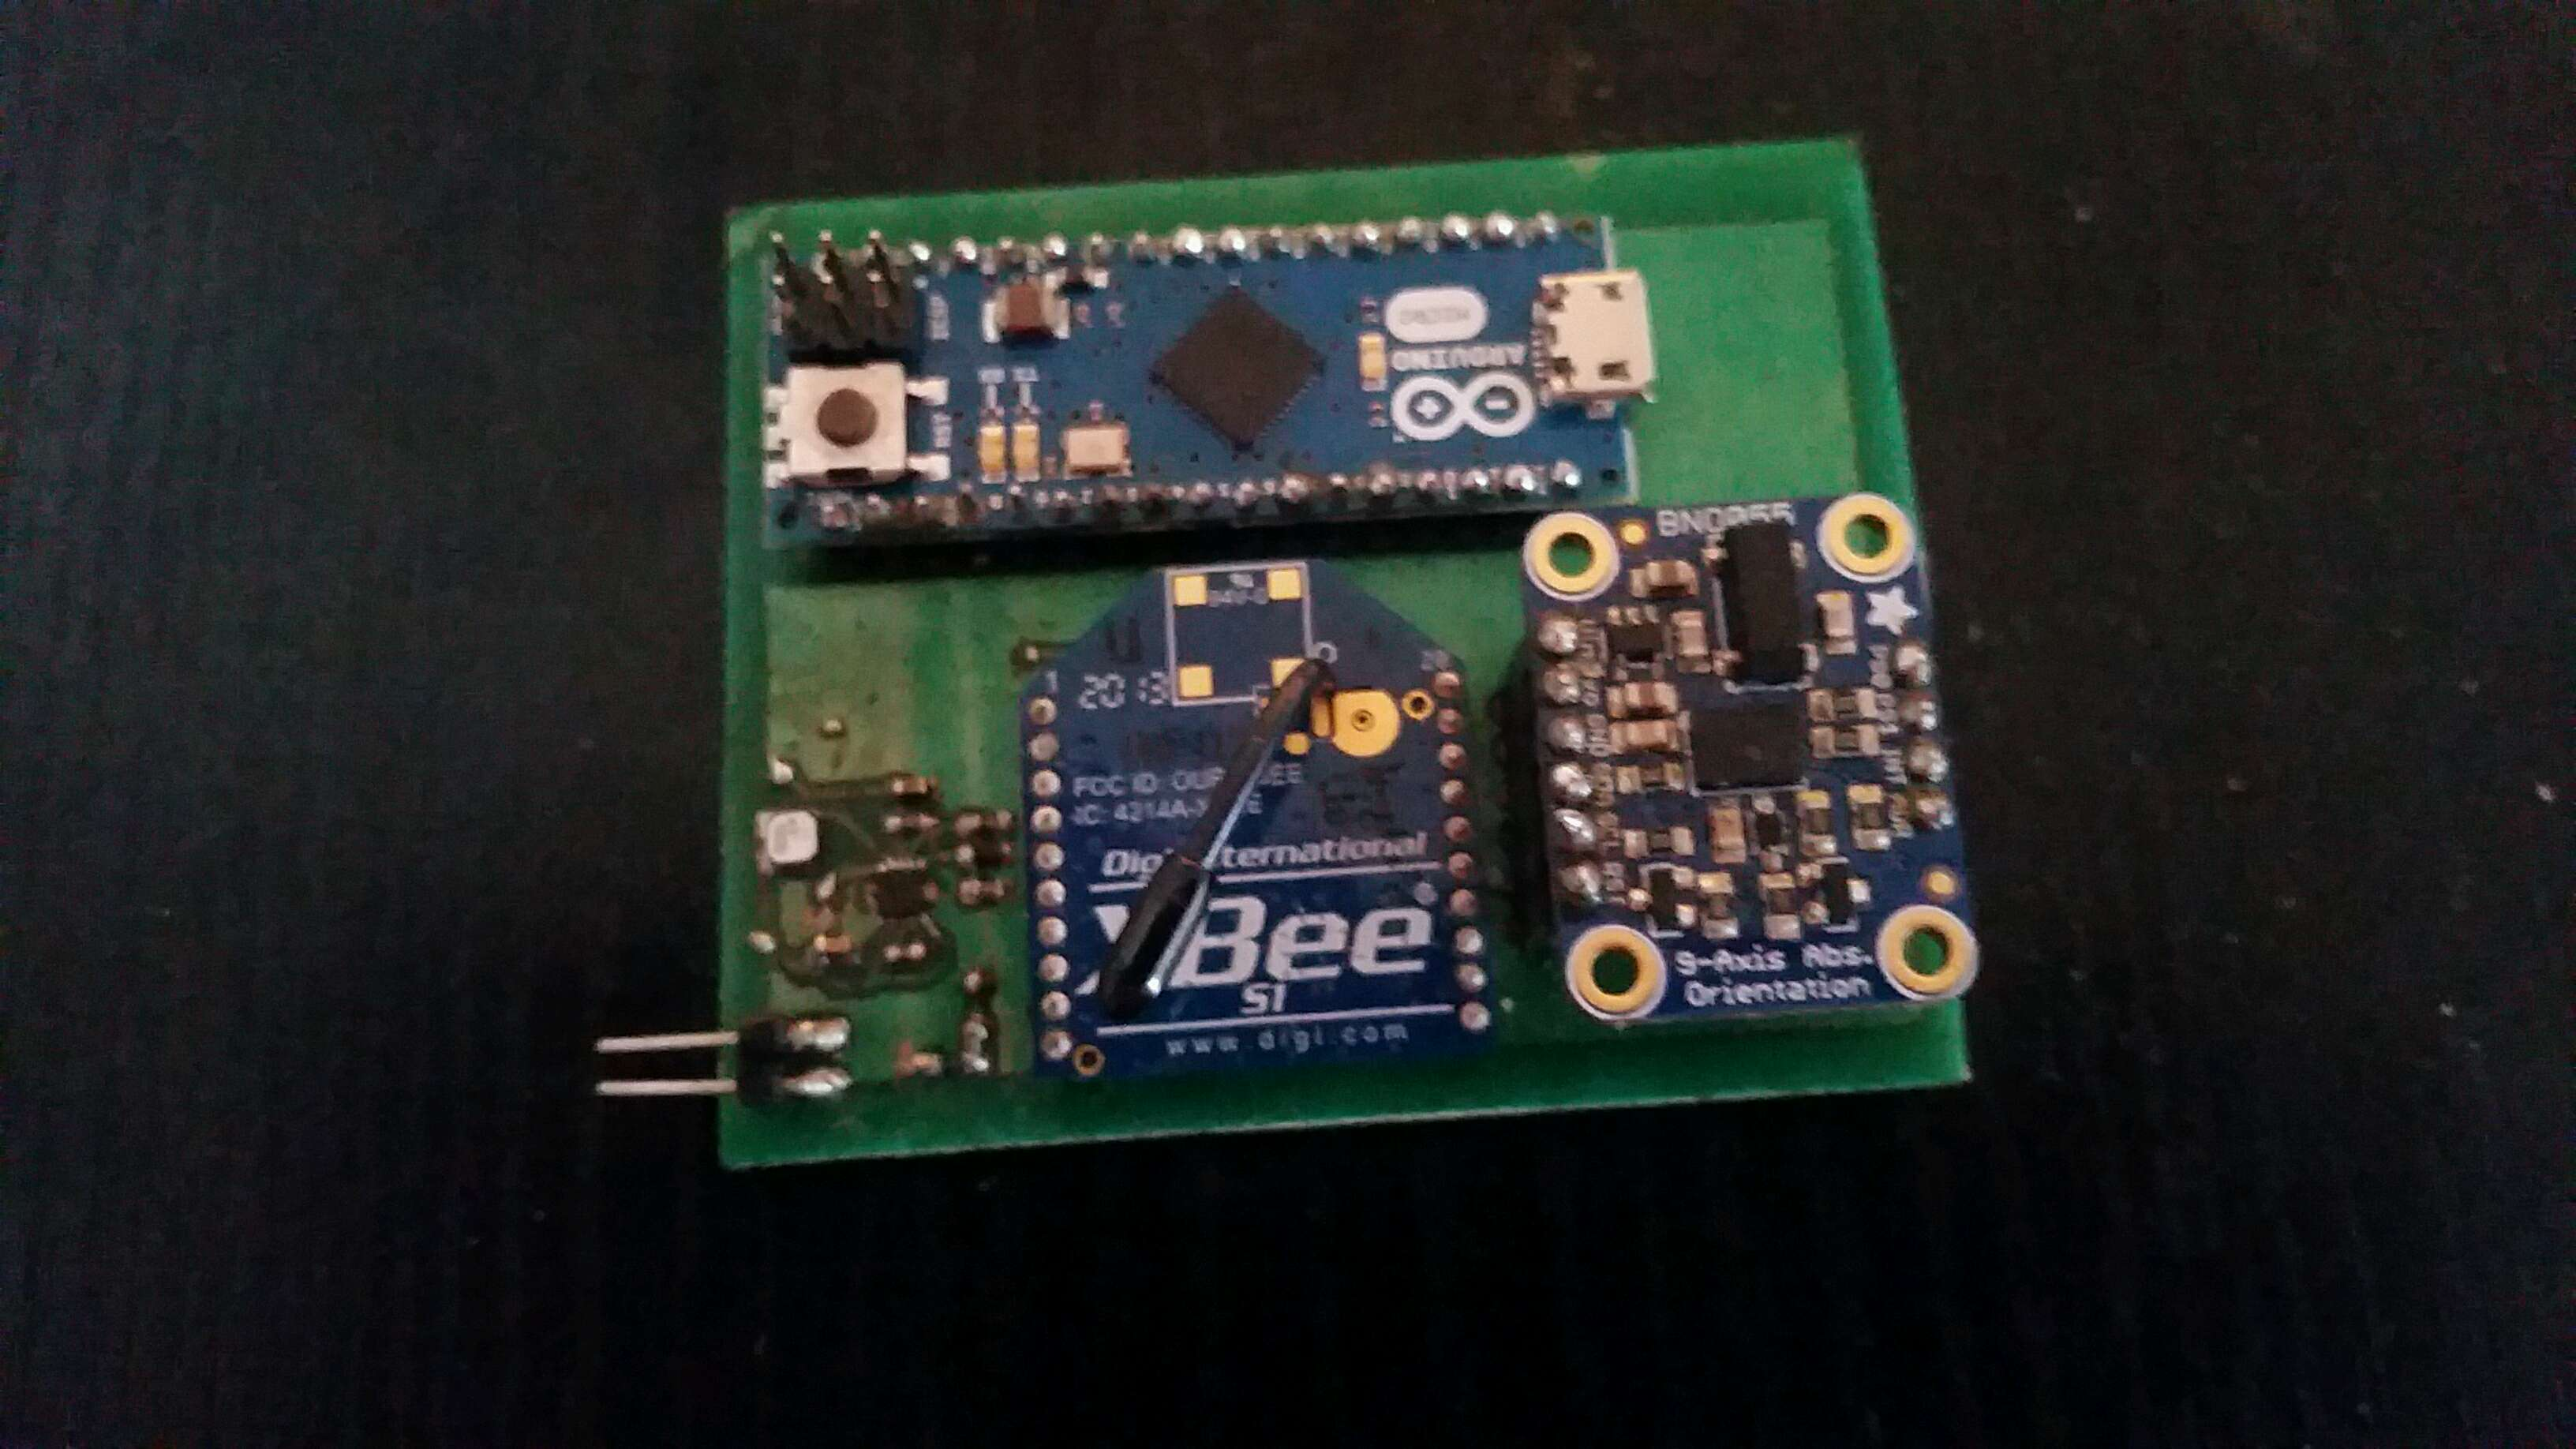
\includegraphics[width=.5\textwidth]{./pictures/placa1}
     	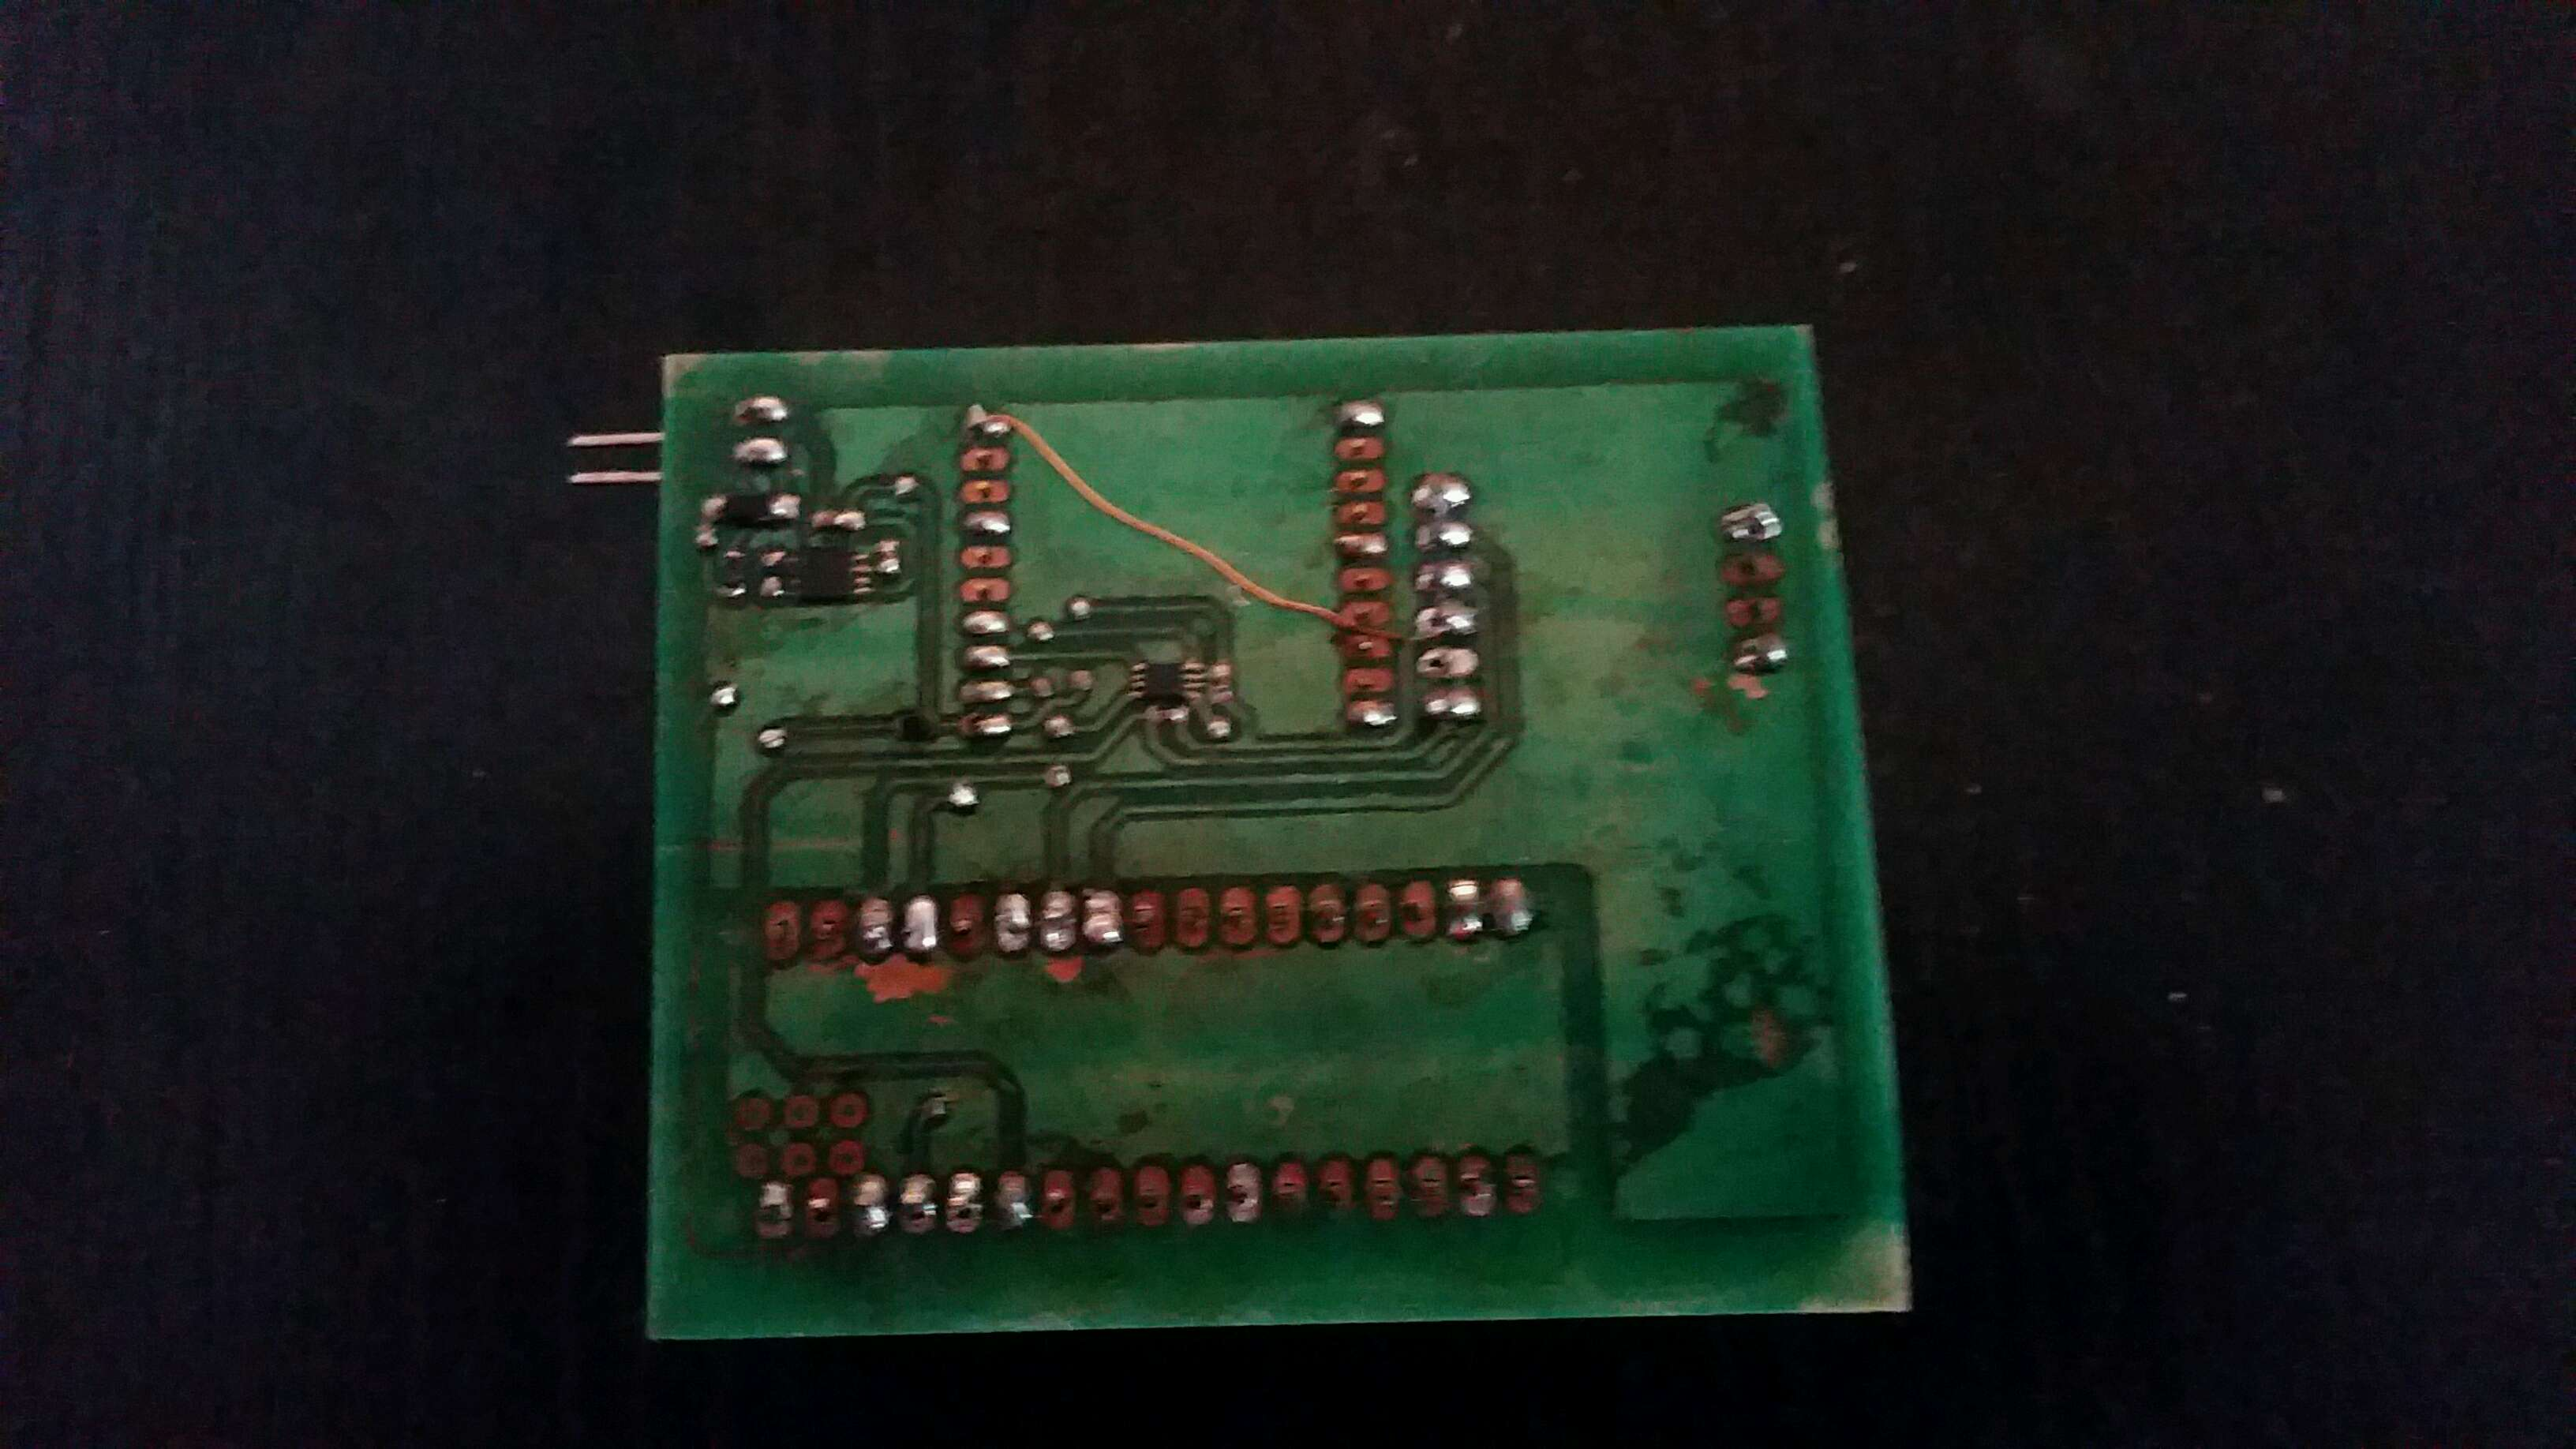
\includegraphics[width=.5\textwidth]{./pictures/placa2}
     	\caption{tarjeta con el IMU}\label{fig: figura}
     \end{figure}
     \begin{figure}[htbp]
     	\centering
     	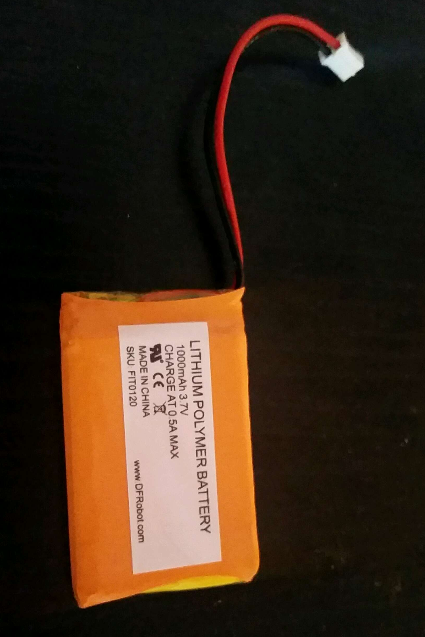
\includegraphics[width=.2\textwidth]{./pictures/pila}
     	\caption{batería recargable}\label{fig: figura}
     \end{figure}
     
     \begin{figure}[htbp]
     	\centering
     	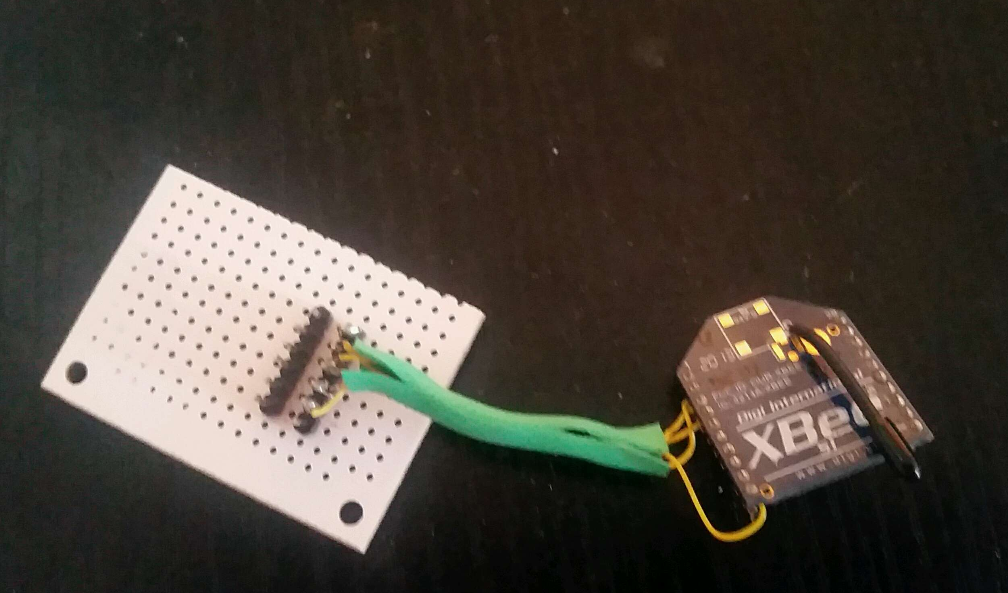
\includegraphics[width=.3\textwidth]{./pictures/placa3}
     	\caption{tarjeta receptora de datos}\label{fig: figura}
     \end{figure}

%*************************************************************************************++
\section{Análisis del comportamiento de los ángulos de mirada $\phi_x$ y $\phi_y$}
Durante la etapa de entrenamiento se requiere capturar bastantes imágenes de personas de frente a la pantalla, con el rostro en diferentes orientaciones debido a que está mirando el objeto en pantalla en diferentes posiciones, para lograr esto se requieren dos cosas durante la etapa de captura de datos:
\begin{itemize}
	\item Se varíe la posición del objeto en pantalla que el sujeto del experimento está observando 
	\item Se debe variar la posición de la persona en el lugar del experimento
\end{itemize}
Sea una instancia de captura de datos la captura de la imagen de una persona anotando su ubicación en el lugar del experimento, la posición del objeto y la orientación de la cabeza (ángulos $\phi_x$ y $phi_y$).
\\Se llega a dar una extensa cantidad de instancias de captura por cada persona variando los parámetros mencionados, lo que llevaría a bastante tiempo de captura de instancias por cada persona y sería muy inconveniente para ellas, por lo tanto se realizó un análisis antes de realizar los experimentos del comportamiento de los ángulos en diferentes circunstancias, el análisis fue realizado mediante el software matemático Octave y a continuación se discuten los resultados.
Suponiendo que es una pantalla ed 42 pulgadas y el marco de referencia se encuentra en la cámara encima de la pantalla.
\begin{itemize}
	\item Ancho de la pantalla: $W=0.9282m$
	\item Largo de la pantalla: $L=0.5523m$
	\item Distancia de la pantalla al piso: $Ly=1.5m$
	\item Distancia de la cámara a la pantalla: $Cy=0.05m$
	\item Estatura del sujeto del experimento: $Hy=1.6m$
	\item Movimiento de la persona a través del eje $Z$: de $0.1m$ a $3m$ con pasos de $0.51786m$
	\item Movimiento de la persona a través del eje $X$: de $-3m$ a $3m$ con pasos de $0.109m$
	\item Movimiento de la figura en pantalla a través del eje $X$: de $-\frac{W}{2}m$ a $\frac{W}{2}m$ con pasos de $0.01658m$
	\item Movimiento de la figura en pantalla a través del eje $Y$: de $-Cy$ a $-(Cy+L)m$ con pasos de $0.051786m$
\end{itemize}

\begin{figure}[htbp]
	\centering
	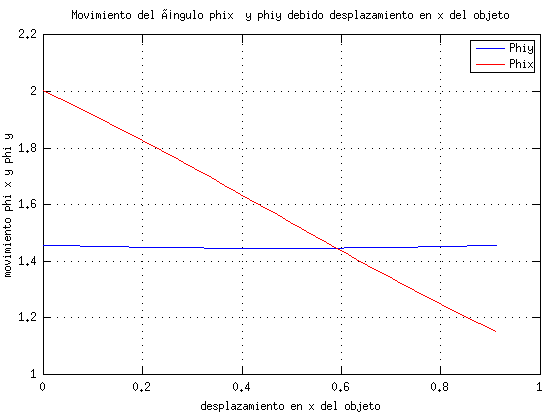
\includegraphics[width=0.6\textwidth]{./pictures/figure1}
	\caption{}\label{fig: figura}
\end{figure}
En la gráfica de la figura 3.1 se puede observar la variación de los ángulos $\phi_x$ y $\phi_y$ con la persona en una única posición: $P=[0, -(L_y+L-H_y), 1]^T$, la variación de la figura en pantalla (en el eje $x$ y $y$) de lo que observan es graficada con el marco de referencia centrado en la esquina superior izquierda de la pantalla, sin embargo los cálculos se hacen tomando la posición de la cámara como marco de referencia. El mayor cambio que ocurre en los ángulos es con respecto a $\phi_x$ de 2 a 1.1 radianes que son 0.9 radianes o 51.5662 grados, lo cual parece tener mucho sentido ya que el desplazamiento se hace en el eje de $\phi_x$. 
\\Lo que resulta peculiar es que a pesar de que no hay desplazamiento en el eje y de la figura  si hay una ligera variación en el ángulo $\phi_y$ de la mirada de la persona, esto se debe al punto de fuga. El punto de fuga es el lugar geométrico en el cual las proyecciones de las rectas paralelas a una dirección dada en el espacio, no paralelas al plano de proyección, convergen, lo anterior se puede ver ilustrado en la figura 3.2, el punto de fuga es el lugar donde convergen todas líneas "paralelas" de color verde, y la línea del horizonte es la recta horizontal de color azul.
\begin{figure}[htbp]
	\centering
	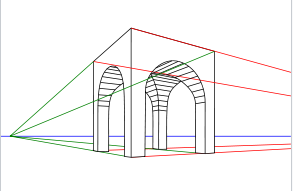
\includegraphics[width=0.3\textwidth]{./pictures/fuga}
	\caption{}\label{fig: figura}
\end{figure}
Cuando la figura inicialmente se encuentra en una posición superior a la de los ojos y se mueve hacia uno de los extremos de la pantalla, ésta pareciera moverse hacia abajo (hacia el horizonte) y cuando inicialmente la figura se encuentra en una posición inferior a la de los ojos de la persona y se mueve hacia un extremo, ésta pareciera moverse hacia arriba por lo tanto la mirada de las personas en el eje $y$ tiende a moverse.

\begin{figure}[htbp]
	\centering
	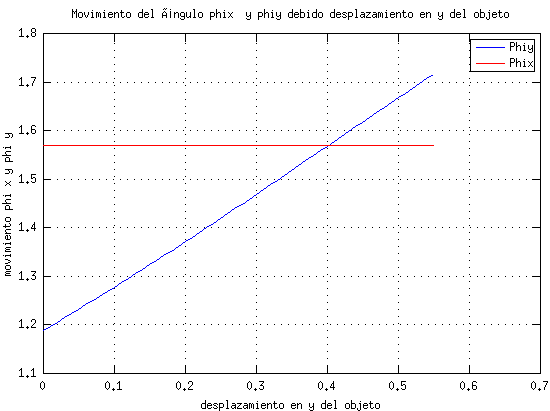
\includegraphics[width=0.6\textwidth]{./pictures/figure2}
	\caption{}\label{fig: figura}
\end{figure}
En la gráfica de la figura 3.3	se puede apreciar que el objeto que observan las personas en pantalla únicamente se desplaza en el eje $y$, en este caso el único desplazamiento de la mirada es con respecto al ángulo  $\phi_y$, al desplazarse el objeto de $0.5523m$ la mirada varía de $1.2$ a $1.7$ radianes, es decir, $0.5$ radianes o lo que e lo mismo $28.6479$ grados.
\begin{figure}[htbp]
	\centering
	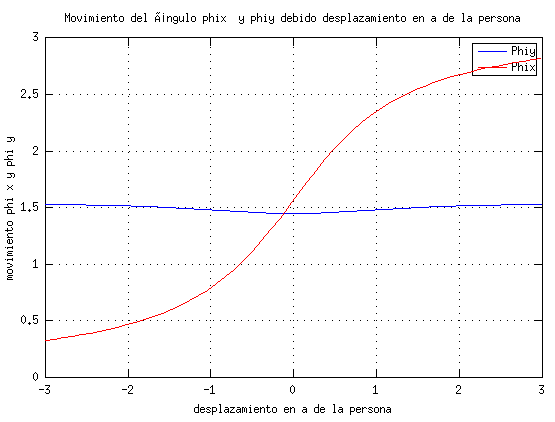
\includegraphics[width=0.6\textwidth]{./pictures/figure3}
	\caption{}\label{fig: figura}
\end{figure}

La gráfica 3.4 describe el caso en el únicamente la  persona se mueve sobre el eje $X$ de $-3$ a $3$m, el mayor desplazamiento lo tiene el ángulo $\phi_x$, de esta gráfica se puede concluir que la mayor variación en el ángulo se da entre $-1$ y $1m$ la cual la mirada varía de $0.8$ a $2.36$ radianes, si la persona se mueve más allá de esta distancia la mirada tiende a estabilizarse y no valdría la pena hacer experimentos en estas zonas. Lo anterior se ve con mayor claridad en la figura 3.5, aquí se amplio el rango en el que se mueve la persona sobre el eje $X$ y en consecuencia $\phi_x$ tiende a estabilizarse.
\begin{figure}[htbp]
	\centering
	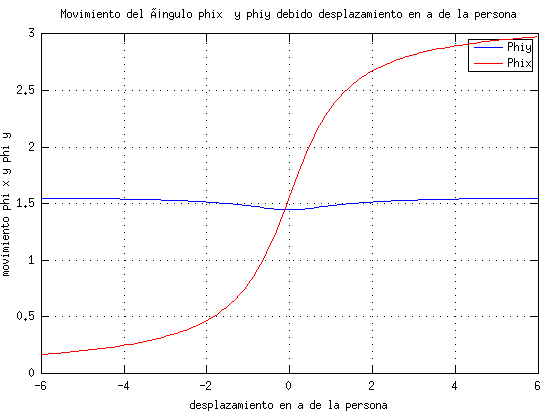
\includegraphics[width=0.6\textwidth]{./pictures/figure5}
	\caption{}\label{fig: figura}
\end{figure}

El último análisis corresponde al caso cuando la figura en pantalla no se mueve y la persona únicamente se mueve sobre el eje $Z$. La figura que observa se encuentra en el centro de la pantalla, es decir en: $[S_x, S_y, S_z]^T=[\frac{W}{2}, -(c_y+\frac{L}{2}), 0]^T$ y la persona se encuentra en $[P_x, P_y, P_z]^T=[0, -(L_y+L-H_y), vecZ]^T$ donde $vecZ$ es un vector que va desde $0.1$ a $3m$.
\begin{figure}[htbp]
	\centering
	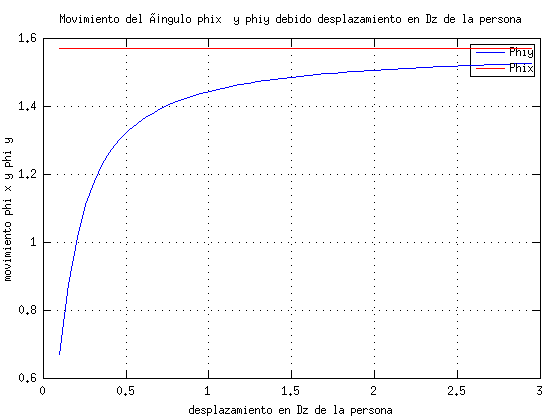
\includegraphics[width=0.6\textwidth]{./pictures/figure4}
	\caption{}\label{fig: figura}
\end{figure}
En la gráfica 3.6 se puede apreciar que mientras se va alejando la persona el único ángulo de la mirada que varía es $\phi_y$, va de $0.6 a 1.55$ radianes, esto quiere decir que hay una variación en el ángulo de 0.95 radianes o 51.56 grados hacia abajo cuando la persona se aleja, además se puede observar que a partir de 1.5m la variación que hay es muy pequeña, de 0 a 0.8m es cuando se da la mayor variación. Lo anterior se puede explicar  con la linea de fuga, mientras la persona se aleja el objeto pareciera moverse hacia abajo y establecer con la mirada de la persona en 1.6 radianes o 91 grados, en el horizonte.

\subsection{Simulación processing}
Se realizó una simulación mediante el software processing del análisis anterior, esto se hizo para poder observar el comportamiento de los ángulos en diferentes posiciones de las personas al mismo tiempo y variar en tiempo real y de manera interactiva la posición en el eje $X$ y $Y$ de la figura en pantalla. Los parámetros del escenario son los mismos a los utilizados en la análisis anterior: $W$, $L$, $LY$, $Cy$ y $Hy$. \\
En la figura 4.1 se puede apreciar una figura de la simulación, en ella se despliegan 36 posiciones de personas separadas por 1m en el eje $X$ y 0.5m en el eje $Y$. La variación en el eje $Y$ se da por medio de la barra deslizante que se encuentra en la esquina inferior derecha, va de 0 a 0.5523m y el desplazamiento en el $Y$ se logra haciendo click en la figura (óvalo blanco) en pantalla que se encuentra en la parte superior de la ventana de la simulación y sin soltar el mouse se arrastra la figura de izquierda a derecha. Los ángulos $\phi_x$ y $\phi_y$ además de ser mostrados en cada una de las posiciones son representados mediante el radio del círculo que representa cada persona y la línea que sale de dicho ángulo, $\phi_x$ es la línea y $\phi_y$ es el radio.\\
\begin{figure}[htbp]
    	\centering
    	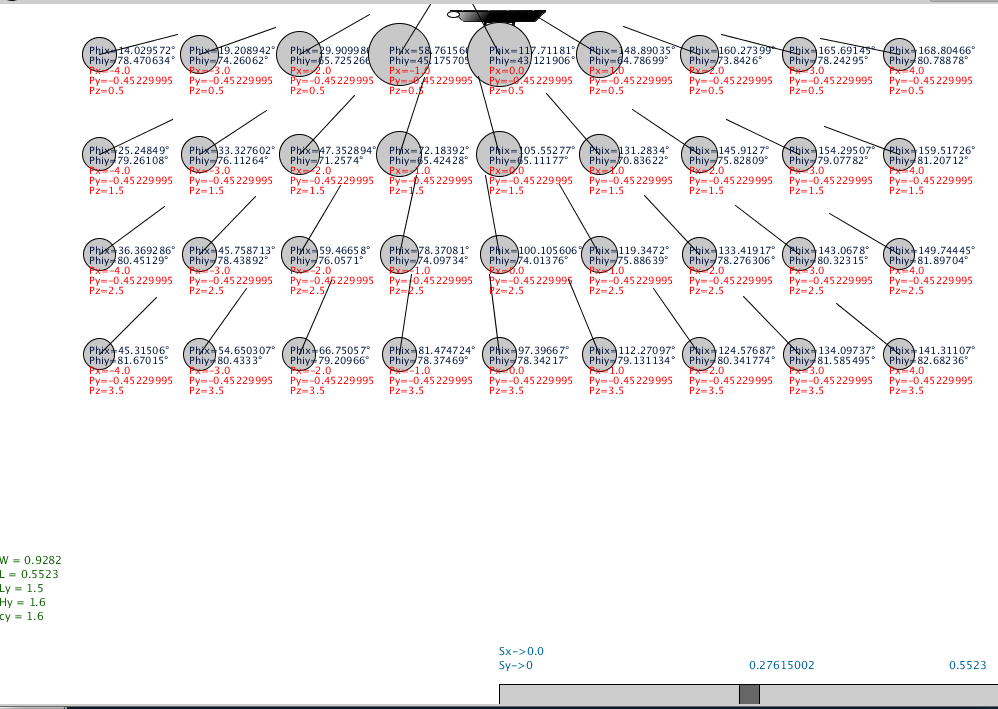
\includegraphics[width=1\textwidth]{./pictures/sim}
    	\caption{}\label{fig: figura}
\end{figure}
Mediante la simulación de igual manera se demostró como al arrastrar la figura únicamente en $X$ no solo varía $\phi_x$ sino también $\phi_y$ de todas las instancias, esto se puede corroborar en los valores de los ángulos y en el área del círculo.

%%****************
\section{Proyeccción de marcas mediante visión computacional, geometría y optimización numérica}
\subsection{Reproyección de punto en la imagen}
	Retomando la sección \ref{repPtsIm} se realizaron experimentos para verificar que la estimación de la rotación y traslación fueran precisos a partir simplemente de la descomposición de la homografía.	El resultado de comprobación se puede ver en la imagen \ref{fig: figRepPtsIm}, las marcas rojas son la proyección en la imagen de la intersecciones con el plano y las verdes son los puntos de $scnPts$ rotados, trasladados y proyectados. Como se puede observar el cálculo de la $n$ y $d$ del plano es bastante precisa, mientras que la $R$ y $T$ tienen error, y parece ser mayor en el desplazamiento sobre el eje $Y$. 
	\begin{figure}[htbp]
		\centering
		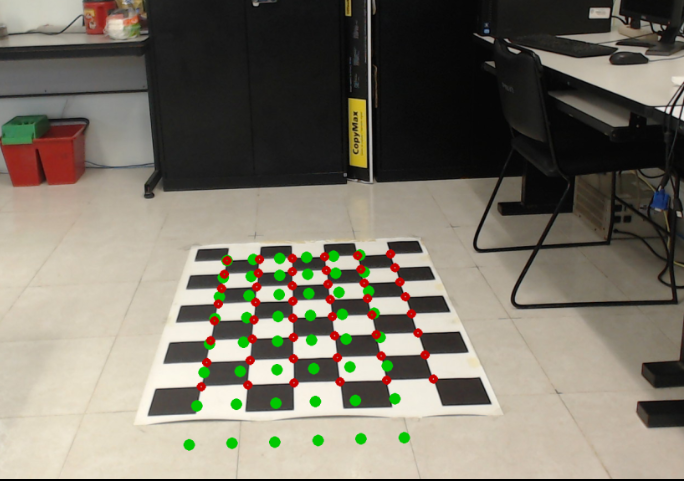
\includegraphics[width=.5\textwidth]{./pictures/rep}
		\caption{Reproyección de puntos} \label{fig: figRepPtsIm}
	\end{figure}
	
	Se realizó un análisis de la distancia que hay entre los que se obtiene de los puntos rotados, traslados y proyectados con lo que debiera ser ($imgPts$) en pixeles y se obtuvo que en el primer punto (primera fila de arriba a abajo y la primera columna de izquierda a derecha): 0.27 pixeles de diferencia en el eje $x$ y 0.15 en $Y$, en el último punto (fila 8 y columna 6) y la distancia es de: $52$ pixeles en $X$ y 107 en $Y$.\\
	El error en metros en tres dimensiones con con respecto al primer y último punto es el siguiente: en el primer punto hay una distancia de $0.0002978m$ en $X$, $0.00003559m$ en $Y$ y $0.000467m$ en $Z$; y en el último punto $0.265m$ en $X$, $0.0268$ en $Y$ y $0.128m$ en $Z$. Como se puede observar el error se va expandiendo conforme los puntos se alejan del primer punto. El error en $R$ y $T$ es mucho mayor que el que hay en $n$ y $d$ esto se debe a que estos últimos parámetros se calculan con respecto al primer punto el cual como ya se analizó tiene menos error, sin embargo; es necesario que $R$ y $T$ sean más precisos porque se utilizan bastante en etapas posteriores, por lo que es necesario optimizar estos parámetros.
	%los puntos obtenidos y estableciendo la distancia a la que estaban los puntos entre si. La matriz con los puntos reales
	%se pusieron marcas en el piso (en lugar donde se trabajó) en la intersección la distancia se pusieroncreó un software para captura
	
	\subsection{Optimización Levenberg-Marquardt}
	Para evaluar los resultados de aplicar el algoritmo de optimización numérica mencionado en la sección \ref{opNum} se creó un programa tomando en cuenta todos los aspectos de dicha sección, y para probar y comparar la eficiencia se utilizan los mismo 48 puntos. Al programa le toma 20 iteraciones llegar al mínimo con un valor de:
	\begin{eqnarray}
	F(p)=1.588771e^{-3}
	\end{eqnarray}
	%(1-cos(\parallel\omega\parallel))
	%sin(\parallel\omega\parallel)
	Se compararon los resultados del mismo modo que en la sección anterior, midiendo la distancia de los puntos en metros rotados y trasladados con la $R$ y $T$ resultantes de la optimización con lo que en realidad debería ser, esto es, los puntos que resultan de la intersección de la proyección de los puntos con el plano del piso. En el primer punto se obtuvo un error de: en $X$ $-0.00145m$, en $Y$ $0.00594m$ y en $Z$ $0.01289m$. En el último en el cual se notaba más el error de la rotación y traslación, ya con la optimización se obtuvieron los siguientes resultados: en $X$ $0.0449m$, en $Y$ $0.0423m$ y en $Z$ $0.1424m$. La mayor diferencia se puede ver el último punto en la coordenada $X$ ya que pasa de una diferencia de $26.5cm$ a $4cm$.
	\begin{figure}[htbp]
		\centering
		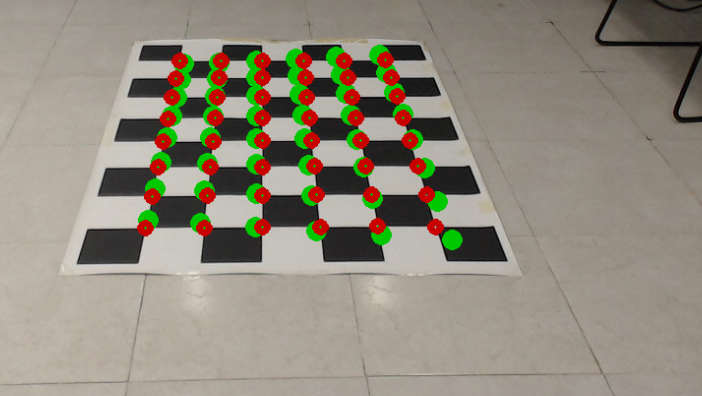
\includegraphics[width=.5\textwidth]{./pictures/conG0}
		\caption{Reproyección de puntos}\label{fig: figura}
	\end{figure}
	En la figura 11.6 se puede apreciar la comparación de los puntos después de optimizar y los resultados son superiores a comparación de lo que hay antes de la optimización.
	
	Sin embargo, en el último punto (esquina inferior derecha)
	
	\subsection{Correción de la imagen y recalibración de la cámara}
	Como se busca que la proyección de los puntos 3d en la imagen con los puntos seleccionados sean lo más precisos posibles se recalibró la cámara (a diferentes resoluciones) con la que se realizan los experimentos mediante herramientas de OpenCV y esta vez se corrigió la distorsión de la cámara mediante los coeficientes de distorsión obtenidos de la recalibración. Todo lo anterior es con el objetivo de aumentar la precisión de la estimación de la matriz de rotación y el vector de traslación.\\
	\begin{figure}[htbp]
		\centering
		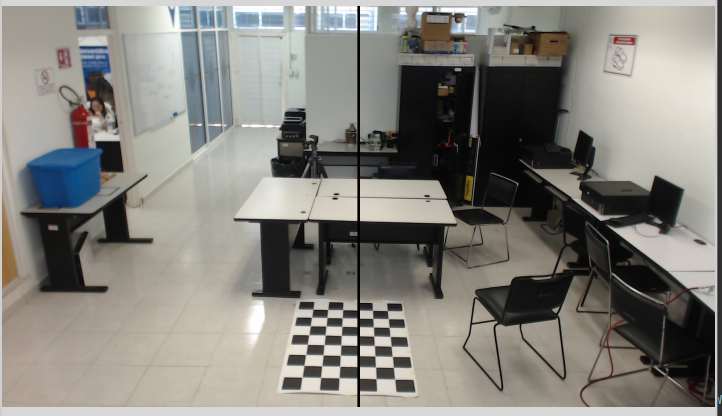
\includegraphics[width=.47\textwidth]{./pictures/p1}
		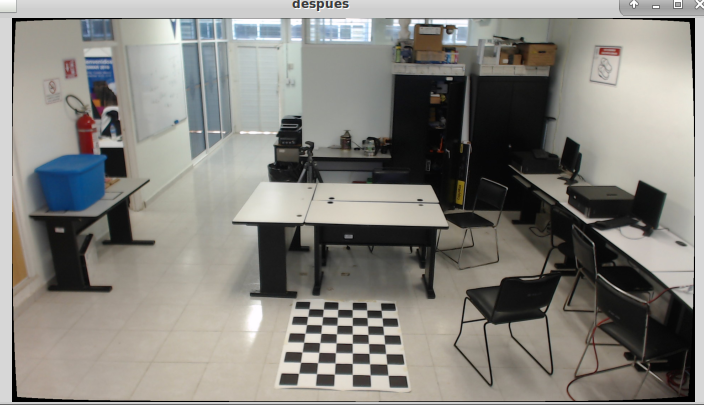
\includegraphics[width=.47\textwidth]{./pictures/p2}
		\caption{Corrección de la imagen}\label{fig: figura}
	\end{figure}
	En la imagen de la izquierda de la figura 4.26 se puede apreciar la imagen antes de la corrección y en la de la derecha con la correción aplicada.\\
	Después de aplicar lo anterior (recalibración y corrección de la cámara) y antes de optimizar se obtienen resultados muy superiores a los conseguidos hasta ahora, ya que $F(p)=  4.10149e-07$, el resultado de comparar los puntos y dibujarlos se puede apreciar en la figura \ref{correctEst}.\\
	\begin{figure}[htbp]
		\centering
		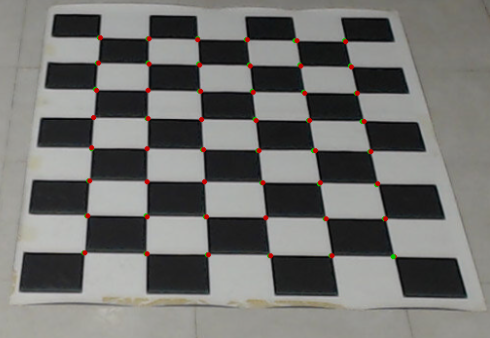
\includegraphics[width=.47\textwidth]{./pictures/correc1}
		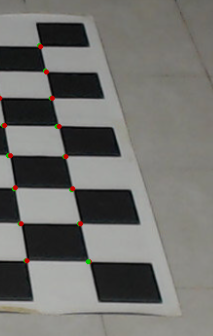
\includegraphics[width=.21\textwidth]{./pictures/correc2}
		\caption{Estimación de R y T antes de la optimización}\label{fig: figura}
		\label{correctEst}
	\end{figure}
	Aplicando nuevamente la optimización numérica a partir del resultado anterior da resultados aún mejores ya que después de 1000 iteraciones se obtiene un mínimo de  $F(p)=  2.908337e-10$ y el resultado gráfico se ve en la imagen \ref{correctEstOpt}.
	%Colocar en el marco teórico como funciona la correción de la distorsión y la calibración
	\begin{figure}[htbp]
		\centering
		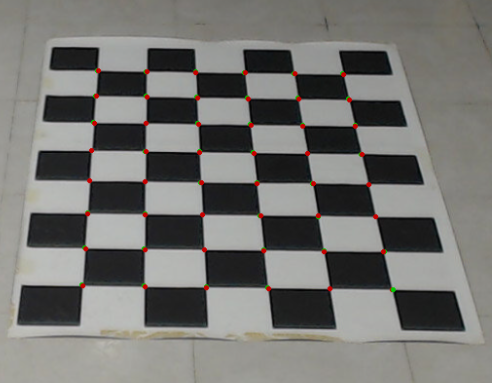
\includegraphics[width=.47\textwidth]{./pictures/correcOpt1}
		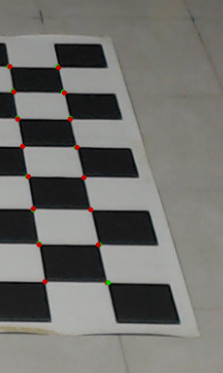
\includegraphics[width=.22\textwidth]{./pictures/correcOpt2}
		\caption{Estimación de R y T después de la optimización p}\label{fig: figura}
		\label{correctEstOpt}
	\end{figure}

\section{Protocolo de captura de datos}
En este punto del proyecto de tesis ya se han descrito casi todos los elementos para realizar la captura de datos:
\begin{itemize}
	\item Estimación del plano del piso a través de la matriz de rotación y traslación optimizadas
	\item Identificación 3D de la ubicación del rostro de las personas y de la figura que observan en pantalla
	\item Ecuaciones para describir el ángulo de la mirada
	\item Generación de secuencia de instancias (marcas en el piso) óptimas para la captura
\end{itemize}
Sin embargo aún falta describir el proceso de captura de datos, los cuales serán utilizados en el algoritmo de entrenamiento. 
\subsection{Proyección en tiempo real de instancias óptimas para marcar en el piso}
El protocolo de captura comienza marcando en el piso las instancias óptimas obtenidas mediante el algoritmo descrito en la sección \ref{secGen}, para ello se desarrolló un programa que recibe como entrada las instancias de marcas, las proyecta y pinta en tiempo real sobre lo que esté capturando la cámara, esto se realiza como guía para o referencia al momento de marcarlas físicamente en el piso del laboratorio de experimentación.\\

Como se ha mencionado los puntos se eligieron tomando en cuenta una región limitada en base a análisis previos y con la restricción (entre otras) de que el rostro de la persona $P$ estuviera dentro del campo visual de la cámara. Esto significa que pudieran darse marcas en el piso $F$ que no se encuentran dentro del campo visual de la cámara, por ejemplo aquellas que se encuentran más cercanas a la cámara, imagen \ref{fig: figVisualFieldIm}.
	\begin{figure}[htbp]
		\centering
		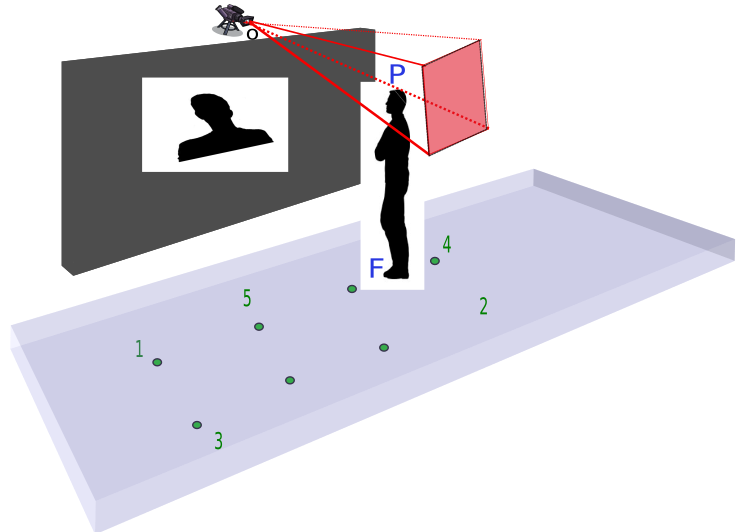
\includegraphics[width=.47\textwidth]{./pictures/visualFieldIm}
		\caption{Campo visual}\label{fig: figVisualFieldIm}
	\end{figure}

\subsubsection{Dibujo de rectas graduadas}
Para solucionar el problema de de instancias F generadas no perceptibles debido a la restricción del campo visual, se desarrolló un algoritmo que utiliza la rotación traslación y parámetros del plano, y dibuja en el piso de la escena las marcas F, en todos los casos se dibujan lineas graduadas paralelas a los ejes $X$ y $Y$ del marco de referencia. A las rectas se les dibuja una pequeña marca cada 10cm, además se dibujan a un lado de las marcas su coordenada 3d. Con esto se busca tomar como referencia las marcas y las rectas graduadas que si se alcanzan a ver y moverse sobre los mismos ejes hasta marcar los puntos $F$ del conjunto de instancias que no se alcanzan a ver en pantalla, esto se puede realizar con ayuda de un flexómetro.\\
Al algoritmo se le añadió la opción de simular la altura de los sujetos de experimentación mediante una recta ortogonal al plano del piso, esto se realizó por dos motivos:
\begin{itemize}
	\item Verificar que la estimación de rotación, traslación y plano obtenidos de etapas anteriores son precisos
	\item Corroborar que el rostro de las personas $P$ que vayan a realizar el experimento se encuentra dentro del campo visual de la cámara
\end{itemize}
Los resultados del algoritmo anterior se pueden ver en la figura \ref{fig: figMarcasPiso} y como se puede apreciar hay unas marcas en las que no se alcanza a apreciar la $F$ pero la $P$ si. Las marcas están enumeradas, esto indica el orden que la personad deberá seguir para la captura de sus datos.\\
\begin{figure}[htbp] 
	\centering
	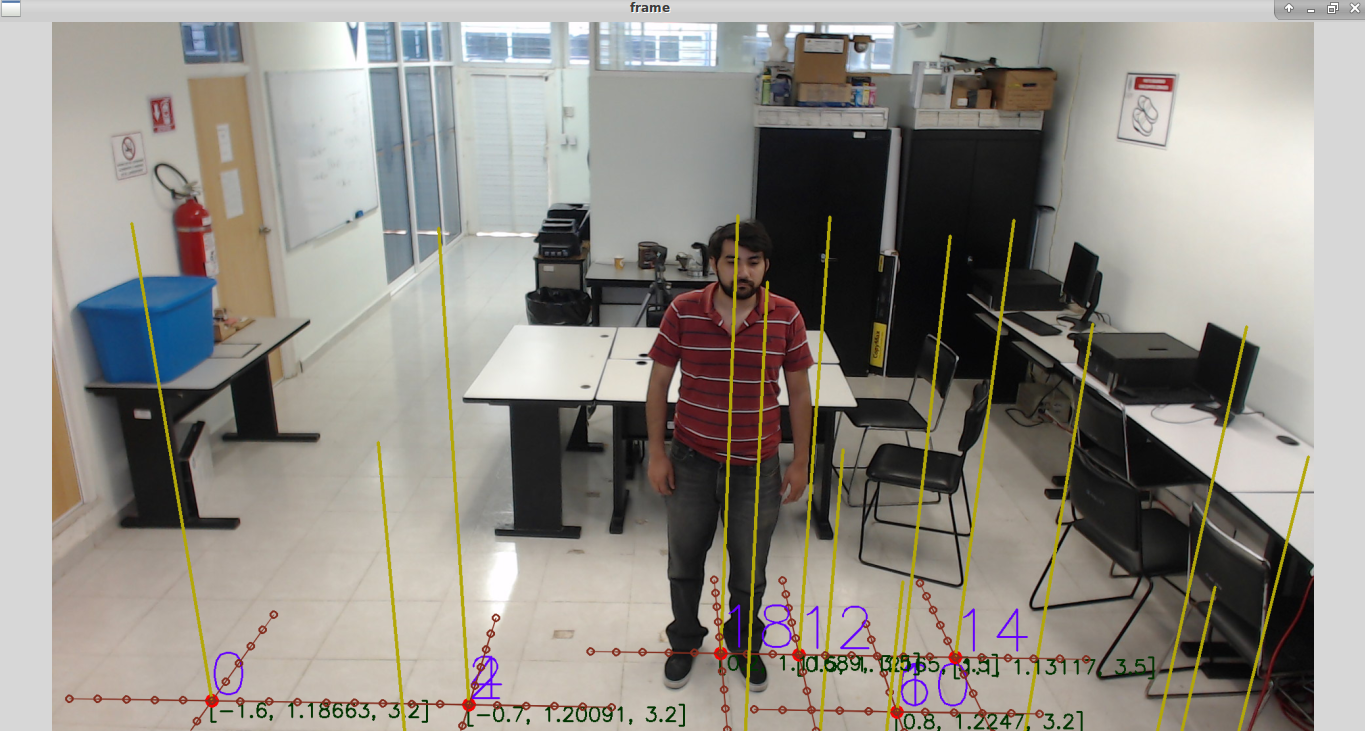
\includegraphics[width=.65\textwidth]{./pictures/marcasPiso}
	\caption{Campo visual}\label{fig: figMarcasPiso}
\end{figure}
La recta amarilla fue colocada y pintada con respecto a la altura real del sujeto de experimentación que aparece en la misma imagen. La orientación de la recta tomando en cuenta que es ortogonal al plano parece estar correcta esto indica que la estimación de la normal del plano $n$ fue estimada con precisión, sin embargo la longitud de la recta se pasa por 3cm.
%¿Explicar como es el algoritmo?

\subsection{Captura de datos}
\begin{figure}[htbp] 
	\centering
	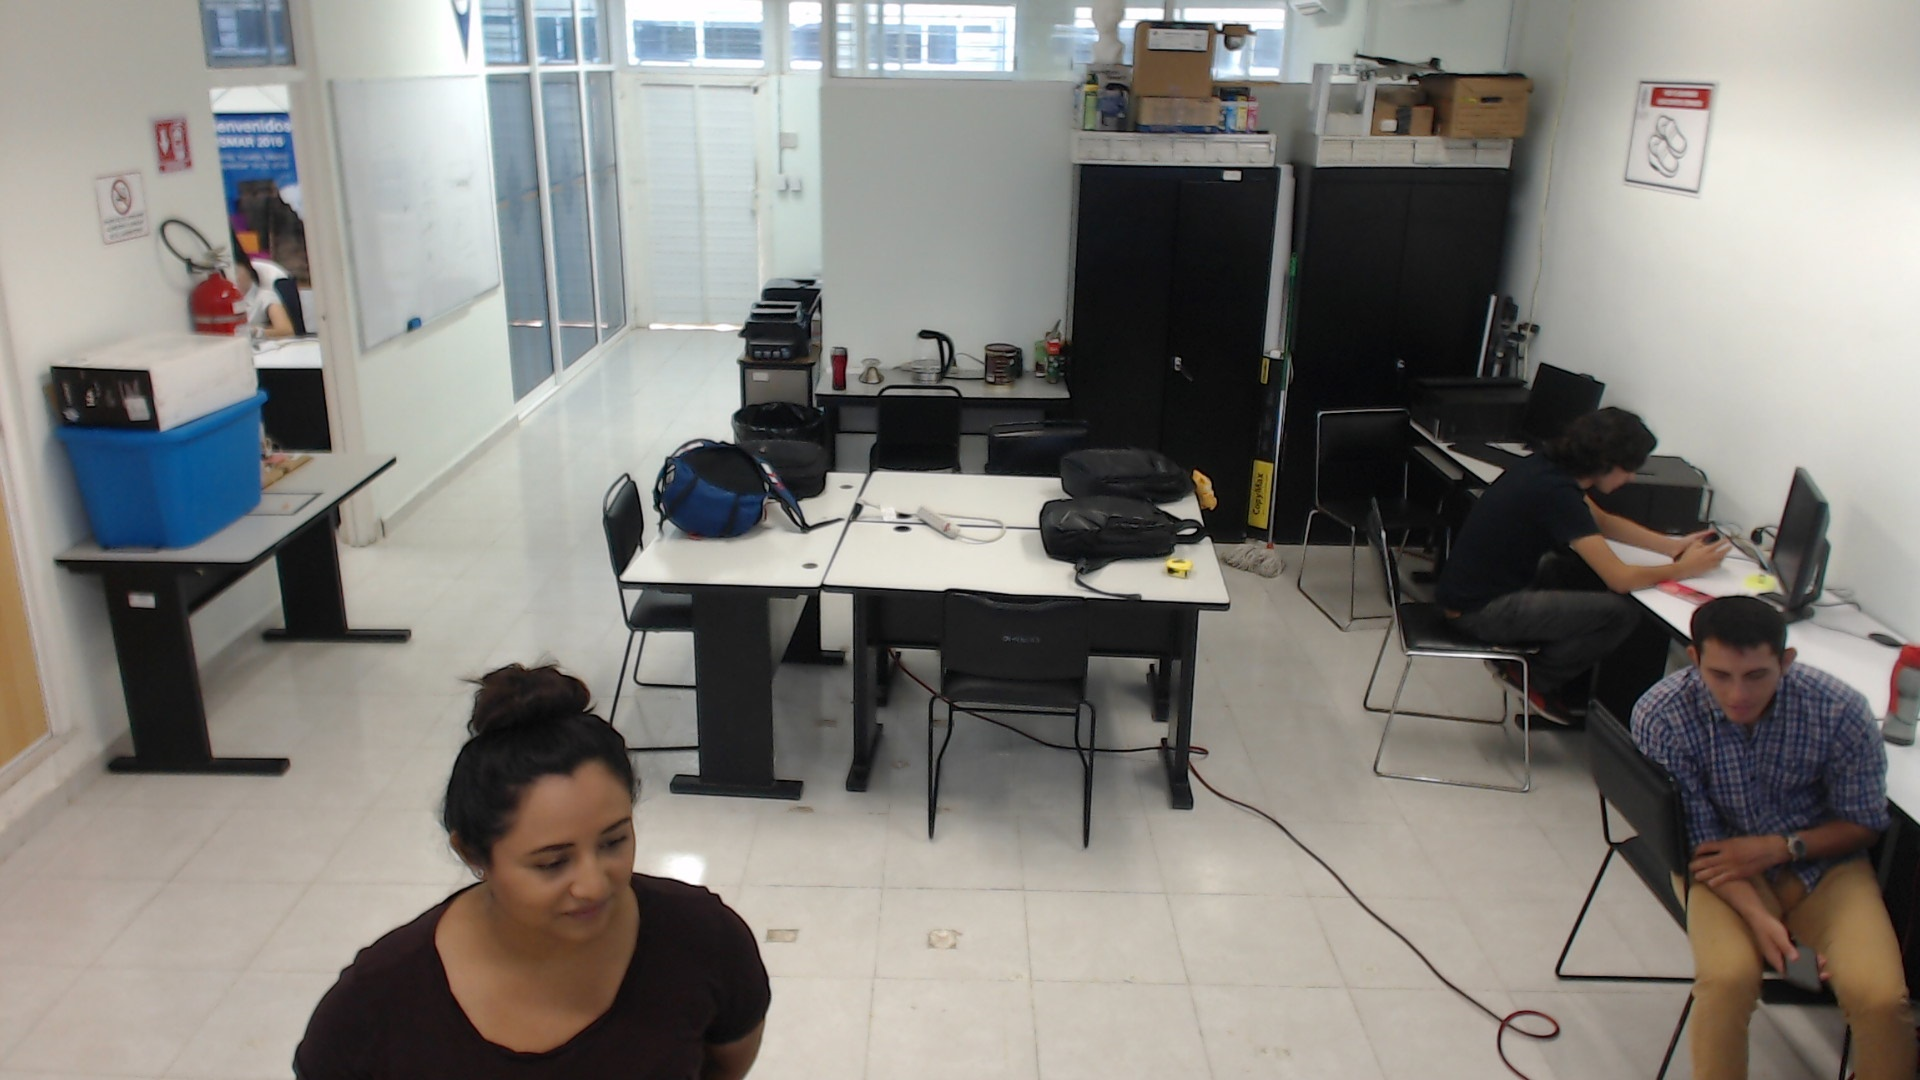
\includegraphics[width=.65\textwidth]{./pictures/mili}
	\caption{Imagen obtenida durante la etapa de captura}\label{fig: figMili}
\end{figure}

\section{Red neuronal}
En la sección se describirá todo lo relacionado a la experimentación de la red neuronal, por ejemplo: la etapa de preparación de datos para introducir a la red, entrenamiento, resultados al variar la topología, etc.
\subsection{Detector de rostros y guardado de los ejemplos útiles}
La primera etapa de esta sección consiste en preparar las imágenes y datos obtenidos de la captura de datos para introducirlos en la red neuronal (incluyendo $P$ y $S$), esto conlleva que en cada imagen se obtenga y guarde la región (ROI) en donde se encuentra el rostro de las personas, por lo tanto se desarrolló un programa con el algoritmo de Viola y Jones para detectar el rostro y guardar la región donde se encuentre. Hay casos en los que a pesar de que el rostro está visible en la imagen, el algoritmo de Viola y Jones no logra detectar el rostro, en este caso descartamos la imagen, ya que para lograr estimar la mirada de las personas con el sistema que se desarrolla es fundamental previamente el rostro con el algoritmo de Viola y Jones.\\
En la figura siguiente \ref{fig: figViola} se pueden ver algunos ejemplos de las imágenes capturadas y procesadas con el detector de Viola y Jones.
\begin{figure}[htbp] 
	\centering
	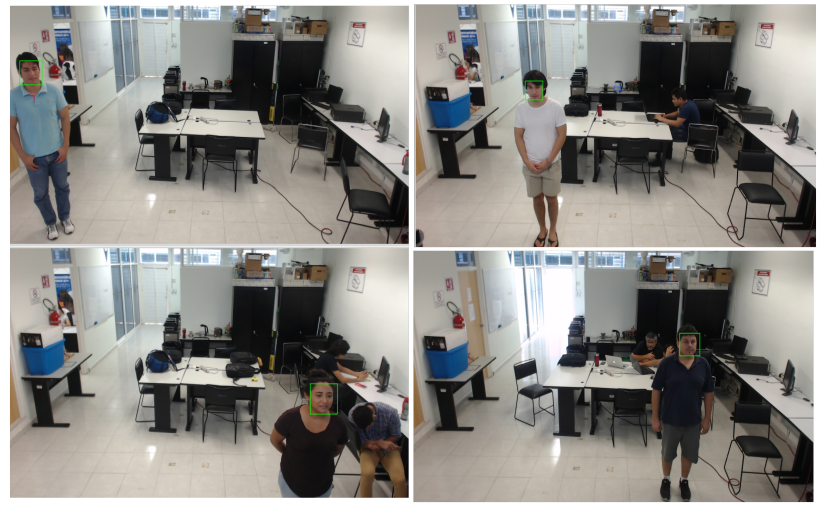
\includegraphics[width=.7\textwidth]{./pictures/violaJones}
	\caption{Imagenes procesadas con Viola y Jones}\label{fig: figViola}
\end{figure}
\\En la imagen  \ref{fig: figNoViola} se presenta un falso positivo del algoritmo detector, el cual es rechazado para el conjunto de entrenamiento.
\begin{figure}[htbp] 
	\centering
	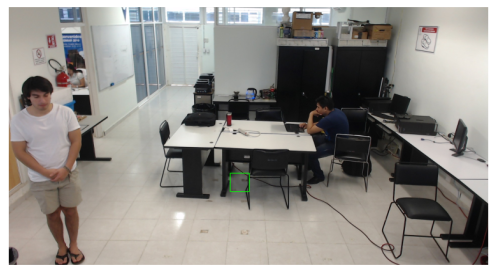
\includegraphics[width=.7\textwidth]{./pictures/noViola}
	\caption{Imagen procesada con Viola y Jones}\label{fig: figNoViola}
\end{figure}
Del total de las 383 después de procesarlas con el detector se obtuvieron 244 rostros útiles para el conjunto de entrenamiento. En la figura \ref{fig: figFacesLab} se encuentran algunos de los rostros que si se utilizan para el conjunto de entrenamiento.
\begin{figure}[htbp] 
	\centering
	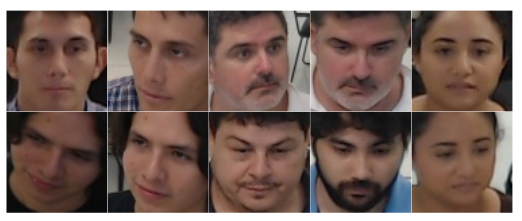
\includegraphics[width=.5\textwidth]{./pictures/facesLab}
	\caption{Imágenes de los rostros guardadas}\label{fig: figFacesLab}
\end{figure}
Las resoluciones de los rostros capturados son muy variadas, pero como se mencionó en la sección \ref{inFeature}, se deben redimensionar todas a un estándar, ya que el número de características y neuronas de entrada depende de la resolución de las imágenes. La resolución elegida para estas pruebas fue de: 75x75.
\subsection{Entrenamiento}
Ya con los datos listos para el entrenamiento se dividen en dos conjuntos, el de entrenamiento y el de prueba, en una primera iteración se probó con x imágenes o ejemplos de entrenamiento y y de prueba. 